\section{トランジスタのDC特性(基本特性)について(原理・計算)}
NPNトランジスタ回路の原理図を図\ref{npn_genri}に示す。
\begin{figure}[htbp]
  \begin{center}
  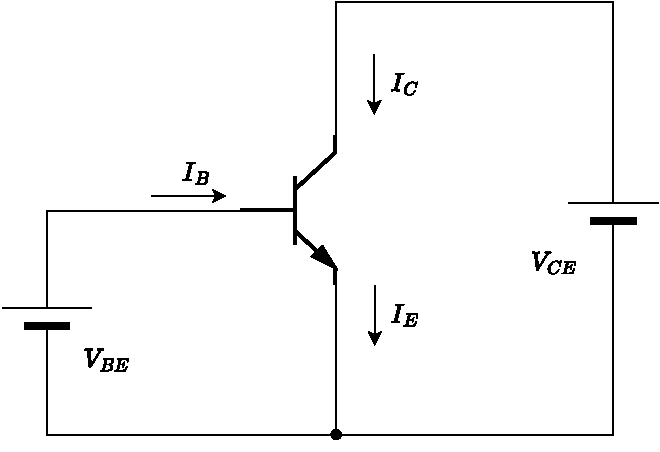
\includegraphics[width=0.5\linewidth]{img/24.pdf}
  \caption{NPNトランジスタ回路の原理図}
  \label{npn_genri}
  \end{center}
\end{figure}
\\キルヒホッフの電流測より、
\begin{align}
  I_E = I_B+I_C  
\end{align}

エミッタ接地直流増幅率を $\beta_0$ とすると、
\begin{align}
  I_C = \beta_0I_B  
\end{align}

また、ベース \- エミッタ間はpn接合ダイオードなので、エミッタ電流 $I_E$ は、
\begin{align}
  I_E \approx I_S\left[\exp\left(\frac{q}{kT}V_{BE}\right)-1\right]\approx I_S\exp\left(\frac{q}{kT}V_{BE}\right)  
\end{align}

$I_S$はダイオードに逆方向の電圧がかかったときの微小な電流(1pA ~ 1nA)である。(図\ref{vbe_ie}を参照。)
$q$ は、電子の負荷、$k$ はボルツマン定数、
Tは絶対温度であり、$\frac{q}{kT}$ の値は、常温(300K)で約 38.7 V$^{-1}$ となる。
式を変形して、
\begin{align}
  & \ln I_E \approx \ln I_S + \frac{q}{kT}V_{BE}\\
  & \log I_E \approx \log I_S + \left(\frac{q}{kT}\log e\right)\cdot V_{BE}
\end{align}
となる。